\PassOptionsToPackage{table,dvipsnames}{xcolor}
\documentclass[10pt,aspectratio=169]{beamer}

%% =================================================================
%%  Theme & colour palette
%% =================================================================
\usetheme[progressbar=frametitle, numbering=fraction, sectionpage=progressbar]{metropolis}
\usefonttheme{professionalfonts}

\definecolor{kaustblue}{RGB}{0, 113, 159}
\definecolor{kaustteal}{RGB}{0, 152, 165}
\definecolor{kaustgold}{RGB}{220, 162, 14}
\definecolor{accent}{RGB}{217, 80, 64}
\definecolor{darkbg}{RGB}{30, 36, 50}

\setbeamercolor{frametitle}{bg=kaustblue, fg=white}
\setbeamercolor{progress bar}{fg=kaustteal, bg=kaustteal!30}
\setbeamercolor{title separator}{fg=kaustteal}
\setbeamercolor{block title}{bg=kaustblue, fg=white}
\setbeamercolor{block body}{bg=kaustblue!8}
\setbeamercolor{alerted text}{fg=accent}
\setbeamercolor{example text}{fg=kaustteal}

%% =================================================================
%%  Packages
%% =================================================================
\usepackage{amsmath, amssymb, amsthm, mathtools}
\usepackage{graphicx}
\usepackage{booktabs}
\usepackage{xcolor}
\usepackage{tikz}
\usepackage{tcolorbox}
\tcbuselibrary{theorems, skins}
\usetikzlibrary{arrows.meta, positioning, shapes.geometric, calc, fit, backgrounds}
\usepackage{pifont}
\newcommand{\cmark}{\textcolor{kaustteal!80!black}{\ding{51}}}
\newcommand{\xmark}{\textcolor{accent}{\ding{55}}}

%% =================================================================
%%  Macros
%% =================================================================
\newcommand{\Div}{\operatorname{div}}
\newcommand{\R}{\mathbb{R}}
\newcommand{\E}{\mathbb{E}}
\newcommand{\W}{\mathcal{W}}
\newcommand{\norm}[1]{\left\lVert #1 \right\rVert}
\newcommand{\eps}{\varepsilon}
\newcommand{\highlight}[1]{\textcolor{accent}{\textbf{#1}}}
\newcommand{\teal}[1]{\textcolor{kaustteal}{#1}}
\newcommand{\gold}[1]{\textcolor{kaustgold}{#1}}
\newcommand{\blue}[1]{\textcolor{kaustblue}{#1}}
\newcommand{\citehl}[1]{\textcolor{kaustblue!80!black}{\textbf{[#1]}}}

%% Pretty boxed result display
\newtcolorbox{resultbox}[1][]{
  enhanced, colback=kaustblue!8, colframe=kaustblue,
  boxrule=0.6pt, arc=2pt, left=8pt, right=8pt, top=6pt, bottom=6pt,
  fonttitle=\bfseries, coltitle=white, colbacktitle=kaustblue,
  attach boxed title to top left={yshift=-2mm, xshift=4mm},
  boxed title style={arc=2pt, boxrule=0pt}, #1
}

\newtcolorbox{idea}[1][]{
  enhanced, colback=accent!8, colframe=accent,
  boxrule=0.6pt, arc=2pt, left=8pt, right=8pt, top=6pt, bottom=6pt,
  fonttitle=\bfseries, coltitle=white, colbacktitle=accent,
  attach boxed title to top left={yshift=-2mm, xshift=4mm},
  boxed title style={arc=2pt, boxrule=0pt}, #1
}

\newtcolorbox{recap}[1][]{
  enhanced, colback=kaustteal!8, colframe=kaustteal,
  boxrule=0.6pt, arc=2pt, left=8pt, right=8pt, top=6pt, bottom=6pt,
  fonttitle=\bfseries, coltitle=white, colbacktitle=kaustteal,
  attach boxed title to top left={yshift=-2mm, xshift=4mm},
  boxed title style={arc=2pt, boxrule=0pt}, #1
}

%% =================================================================
%%  Title metadata
%% =================================================================
\title{Deep Learning for Mean Field Games\\with Non-Separable Hamiltonians}
\subtitle{A walk through Assouline \& Missaoui (2023),\\and how our work extends it}
\author{Hikmatullo Ismatov}
\institute{King Abdullah University of Science and Technology\\
           \emph{Joint work with Prof.\ Diogo A.\ Gomes}}
\date{\today}

\begin{document}

%% =================================================================
%%  1. TITLE
%% =================================================================
\begin{frame}[plain]
  \maketitle
\end{frame}

%% =================================================================
%%  2. ROAD MAP
%% =================================================================
\begin{frame}{What this talk covers}
\begin{tcolorbox}[colback=kaustteal!8, colframe=kaustteal, arc=3pt]
\centering\large
We will read the paper of \blue{Assouline \& Missaoui (2023)} together\\
and connect it to a new method we are developing.
\end{tcolorbox}

\vspace{0.3cm}
\textbf{Plan:}
\begin{enumerate}\setlength\itemsep{2pt}
  \item Foundations: \emph{what is a Mean Field Game?}
  \item Why solving them is hard in high dimensions
  \item Two families of deep solvers: \emph{GAN-based} and \emph{physics-informed}
  \item Background tools: \emph{GANs}, \emph{Hopf formula}, \emph{APAC-Net}
  \item The paper: \emph{MFDGM} of Assouline \& Missaoui
  \item Convergence theory and experiments
  \item \alert{Our contribution}: Extended-MFGAN with explicit rate
\end{enumerate}

\medskip
\begin{center}
\teal{Every term will be defined before it is used. Please interrupt at any time.}
\end{center}
\end{frame}

%% =================================================================
%%  PART 1 -- FOUNDATIONS
%% =================================================================
\section{\texorpdfstring{Part 1 \;\textbar\; Foundations}{Part 1 | Foundations}}

\begin{frame}{What is a Mean Field Game? \;\textnormal{\small(intuition)}}
\textbf{Picture this.} A thousand drivers on the same highway.
\smallskip
\begin{itemize}\setlength\itemsep{1pt}
  \item Each driver wants to reach their destination quickly.
  \item Where the road is \alert{crowded}, everyone slows down.
  \item Where it's \teal{empty}, everyone speeds up.
\end{itemize}

\medskip
So each driver's best strategy depends on \alert{what everyone else does},
and everyone else's strategy depends on each driver. \emph{Circular.}

\medskip
\begin{idea}[title={Mean Field Game (\citehl{Lasry--Lions 2007}, \citehl{Huang--Caines--Malham\'e 2006})}]
The mathematical theory that resolves this circularity, by finding a
\emph{Nash equilibrium}: a strategy from which no single agent benefits
by deviating alone.
\end{idea}

\medskip
\teal{``Mean field''} because no individual agent matters, only the
\emph{average behaviour} (the density) of the crowd.
\end{frame}

\begin{frame}{The two quantities we care about}
At Nash equilibrium, two objects describe everything:

\medskip
\begin{center}
\begin{tabular}{cll}
\toprule
Symbol & Name & What it means \\
\midrule
$\rho(t,x)$ & \blue{population density} & how many agents are at $x$ at time $t$ \\
$\varphi(t,x)$ & \blue{value function} & ``best total cost from now until $T$ if I'm at $x$'' \\
\bottomrule
\end{tabular}
\end{center}

\medskip
\textbf{Intuition for $\varphi$.}  Think of $\varphi$ as a
\teal{map of regret}: it answers, \emph{``if I'm at $x$ at time $t$ and
I play optimally from now on, how much cost do I accumulate?''}

\medskip
$\rho$ is observable in the world. $\varphi$ lives inside each agent's head.
\end{frame}

\begin{frame}{The MFG system (\citehl{Lasry--Lions 2007})}
\textbf{Backward HJB equation} (governs $\varphi$, runs from $t=T$ to $t=0$):
\[
  -\partial_t\varphi - \nu\Delta\varphi + H(x, \rho, \nabla\varphi) = 0
\]

\textbf{Forward Fokker--Planck equation} (governs $\rho$, runs from $t=0$ to $t=T$):
\[
  \partial_t\rho - \nu\Delta\rho - \Div\!\bigl(\rho\,\nabla_p H(x, \rho, \nabla\varphi)\bigr) = 0
\]

\smallskip
\textbf{Boundary conditions.}
$\rho(0,x) = \rho_0(x)$ \;(initial crowd), \;
$\varphi(T,x) = g(x, \rho(T,x))$ \;(terminal cost).

\vspace{0.3cm}
\begin{center}
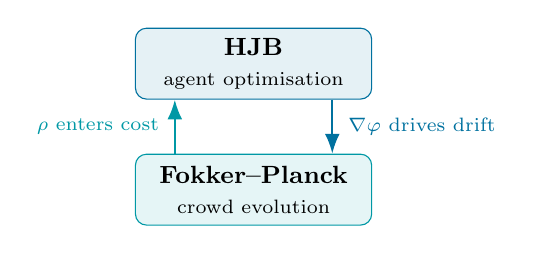
\begin{tikzpicture}[font=\small]
  \node[draw=kaustblue, fill=kaustblue!10, rounded corners, minimum width=3cm, minimum height=0.9cm, align=center] (HJB) at (0,1.2) {\textbf{HJB}\\\scriptsize agent optimisation};
  \node[draw=kaustteal, fill=kaustteal!10, rounded corners, minimum width=3cm, minimum height=0.9cm, align=center] (FP) at (0,-0.4) {\textbf{Fokker--Planck}\\\scriptsize crowd evolution};
  \draw[-{Latex[length=2.5mm]}, kaustblue, thick]
       ([xshift=1cm]HJB.south) -- node[right=2pt, font=\scriptsize, kaustblue]
       {$\nabla\varphi$ drives drift} ([xshift=1cm]FP.north);
  \draw[-{Latex[length=2.5mm]}, kaustteal, thick]
       ([xshift=-1cm]FP.north) -- node[left=2pt, font=\scriptsize, kaustteal]
       {$\rho$ enters cost} ([xshift=-1cm]HJB.south);
\end{tikzpicture}
\end{center}

\smallskip
The two equations are \alert{coupled}.  Solving them \emph{together} is the challenge.
\end{frame}

\begin{frame}{The Hamiltonian $H$ \;\textnormal{\small(don't be scared)}}
The function $H(x, \rho, p)$ is the \blue{Hamiltonian} of the game.
It is just a \emph{cost function in disguise}, defined by
\[
  H(x, \rho, p) \;=\; \sup_{v}\,\bigl\{\,-v\!\cdot\!p \;-\; L(x, \rho, v)\,\bigr\}
  \qquad \text{(Legendre transform)}
\]
where $L$ is the agent's running cost and $v$ is velocity.

\medskip
\textbf{Concrete example.} If $L(x,\rho,v) = \tfrac12|v|^2 - f_0(x,\rho)$, then
\[
  H(x,\rho,p) \;=\; \tfrac12|p|^2 \;-\; f_0(x,\rho).
\]

\medskip
\begin{recap}[title=What you must remember]
$H$ is \emph{known} (given by the modeller).
It packages the running cost into a function of a ``momentum'' $p$.
In the MFG, $p = \nabla\varphi$.
\end{recap}
\end{frame}

\begin{frame}{Separable vs.\ non-separable Hamiltonians}
\textbf{The single most important distinction in the talk.}

\medskip
\begin{columns}[T]
\begin{column}{0.49\textwidth}
\begin{tcolorbox}[colback=kaustteal!8, colframe=kaustteal,
                  title={\textbf{Separable}}, fonttitle=\bfseries]
\[
  H(x,\rho,p) = H_0(x,p) - f_0(x,\rho)
\]
\smallskip
$\rho$ and $p$ appear in \emph{different} terms, never multiplied.

\medskip
\teal{Example:} $H = \tfrac12|p|^2 - \lambda\rho$.
\end{tcolorbox}
\end{column}
\begin{column}{0.49\textwidth}
\begin{tcolorbox}[colback=accent!8, colframe=accent,
                  title={\textbf{Non-separable}}, fonttitle=\bfseries]
\[
  H(x,\rho,p) = ?
\]
\smallskip
$\rho$ and $p$ are \alert{mixed} (multiplied together).

\medskip
\alert{Example:} traffic flow (\citehl{Huang et al.\ 2019})
\[
  H = \tfrac12|p|^2 - (1-\rho)\,p
\]
\end{tcolorbox}
\end{column}
\end{columns}

\medskip
\begin{center}
\textbf{Why this matters.}  Some deep-learning methods need separability.\\
When $\rho$ and $p$ are entangled, those methods \emph{break}.
\end{center}
\end{frame}

%% =================================================================
%%  PART 2 -- WHY HARD
%% =================================================================
\section{\texorpdfstring{Part 2 \;\textbar\; Why is this hard?}{Part 2 | Why is this hard?}}

\begin{frame}{The curse of dimensionality}
\textbf{Classical PDE solvers} (finite differences) put down a grid.

\smallskip
\begin{center}
\begin{tabular}{rrr}
\toprule
dimension $d$ & grid points $N=100$ per axis & total points $N^d$ \\
\midrule
$1$  & $100$       & $100$ \\
$2$  & $100\times 100$ & $10\,000$ \\
$3$  & $100\times100\times100$ & $10^6$ \\
$10$ & ---         & $10^{20}$ \\
$100$& ---         & \alert{$10^{200}$} \\
\bottomrule
\end{tabular}
\end{center}

\medskip
A 100-dimensional MFG has \alert{$10^{200}$} grid cells.
This is \emph{more than the number of atoms in the universe}.

\medskip
\begin{idea}[title=Curse of dimensionality]
Classical grid-based methods \emph{cannot} solve high-dimensional MFGs.
\end{idea}

\medskip
\textbf{But} many MFG applications (large-scale traffic, financial markets,
multi-agent RL) live in high dimensions.
\end{frame}

\begin{frame}{Neural networks to the rescue}
A \blue{neural network} is a parameterised function $f_\theta(x)$
whose weights $\theta$ can be tuned.

\medskip
\begin{idea}[title=Universal Approximation Theorem (\citehl{Hornik 1991})]
A neural network with a \emph{single} hidden layer and enough neurons
can approximate any continuous function to arbitrary accuracy,
\emph{in any dimension}, without a grid.
\end{idea}

\medskip
\textbf{Strategy.}  Replace the unknowns $\varphi$, $\rho$ with neural
networks $\varphi_\omega$, $\rho_\theta$, and \emph{optimise the weights}
so the networks solve the PDE.

\medskip
The number of parameters of a neural net does \emph{not} explode
with dimension. A $100$-dimensional network with $100$ hidden units has
$\sim 10\,000$ parameters --- entirely tractable.
\end{frame}

\begin{frame}{Two ways to train the networks}
\begin{columns}[T]
\begin{column}{0.49\textwidth}
\begin{tcolorbox}[colback=kaustblue!8, colframe=kaustblue,
                  title={\textbf{Physics-informed / PINN / DGM}},
                  fonttitle=\bfseries]
Plug the network into the PDE and minimise the residual:
\[
  \min_\omega \, \E\bigl[\,|\text{HJB residual}|^2\bigr]
\]
\textbf{Family:} DGM (\citehl{Sirignano--Spiliopoulos 2018}),
PINN (\citehl{Raissi et al.\ 2019}), MFDGM (\citehl{Assouline--Missaoui 2023}).
\smallskip\\
Works for \cmark\;any $H$.
\end{tcolorbox}
\end{column}
\begin{column}{0.49\textwidth}
\begin{tcolorbox}[colback=kaustteal!8, colframe=kaustteal,
                  title={\textbf{Variational / GAN-based}},
                  fonttitle=\bfseries]
Rewrite the PDE as a \emph{saddle-point problem}, then two networks
play a game:
\[
  \min_G \max_D \, L(G,D)
\]
\textbf{Family:} APAC-Net (\citehl{Lin et al.\ 2021}),
MFGAN (\citehl{Ruthotto et al.\ 2020}).
\smallskip\\
Works only for \xmark\;separable $H$.
\end{tcolorbox}
\end{column}
\end{columns}

\medskip
\begin{center}
\textbf{Today's paper sits in the left column.}
\teal{Our work bridges the two columns.}
\end{center}
\end{frame}

%% =================================================================
%%  PART 3 -- GANS
%% =================================================================
\section{\texorpdfstring{Part 3 \;\textbar\; What is a GAN?}{Part 3 | What is a GAN?}}

\begin{frame}{Generative models: the goal}
\textbf{Setup.} I show you a million photos of cats.
\smallskip\\
I ask: write a program that produces \emph{new} cat photos that look real.

\medskip
\textbf{Mathematical version.} Given samples $x_1,\ldots,x_N \sim P_{\text{data}}$
from an unknown distribution, build a program that outputs fresh samples
from $P_{\text{data}}$ (or a close approximation).

\medskip
\textbf{This is the generative modelling problem.}\\[3pt]
\teal{Generative Adversarial Networks} are one solution.
\end{frame}

\begin{frame}{GAN: a two-player game \;\textnormal{(\citehl{Goodfellow et al.\ 2014})}}
\begin{columns}[T]
\begin{column}{0.49\textwidth}
\textbf{The two players.}
\smallskip
\begin{itemize}\setlength\itemsep{2pt}
  \item \blue{Generator $G_\theta(z)$}: takes random noise $z$, outputs a
        \emph{fake sample}.\\
        \emph{Goal:} make fakes that look real.
  \item \teal{Discriminator $D_\omega(x)$}: takes a sample, outputs a
        probability ``is this real?''\\
        \emph{Goal:} catch the fakes.
\end{itemize}
\end{column}
\begin{column}{0.49\textwidth}
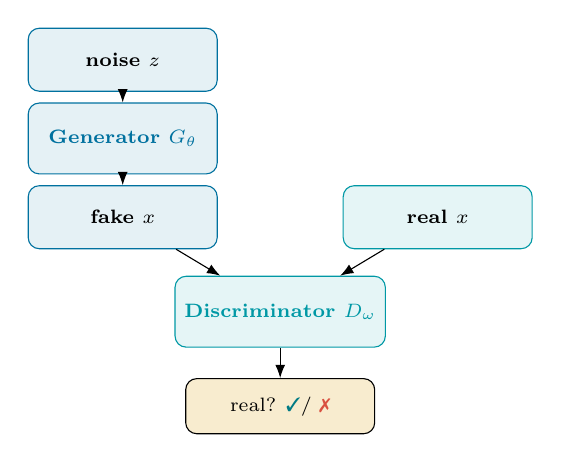
\begin{tikzpicture}[font=\scriptsize]
  \node[draw=kaustblue, fill=kaustblue!10, rounded corners, minimum width=2.4cm, minimum height=0.8cm] (z) at (0,2)
       {\textbf{noise $z$}};
  \node[draw=kaustblue, fill=kaustblue!10, rounded corners, minimum width=2.4cm, minimum height=0.9cm] (G) at (0,1.0)
       {\blue{\textbf{Generator $G_\theta$}}};
  \node[draw=kaustblue, fill=kaustblue!10, rounded corners, minimum width=2.4cm, minimum height=0.8cm] (fake) at (0,0)
       {\textbf{fake $x$}};
  \node[draw=kaustteal, fill=kaustteal!10, rounded corners, minimum width=2.4cm, minimum height=0.8cm] (real) at (4,0)
       {\textbf{real $x$}};
  \node[draw=kaustteal, fill=kaustteal!10, rounded corners, minimum width=2.4cm, minimum height=0.9cm] (D) at (2,-1.2)
       {\teal{\textbf{Discriminator $D_\omega$}}};
  \node[draw, fill=kaustgold!20, rounded corners, minimum width=2.4cm, minimum height=0.7cm] (out) at (2,-2.4)
       {real? \cmark / \xmark};
  \draw[-{Latex}] (z) -- (G);
  \draw[-{Latex}] (G) -- (fake);
  \draw[-{Latex}] (fake) -- (D);
  \draw[-{Latex}] (real) -- (D);
  \draw[-{Latex}] (D)    -- (out);
\end{tikzpicture}
\end{column}
\end{columns}

\medskip
\textbf{Game-theoretic objective:}
\[
  \min_G \;\max_D\;
  \bigl\{\,
    \E_{x\sim P_{\text{data}}}\!\bigl[\log D(x)\bigr]
    \;+\;
    \E_{z\sim P_z}\!\bigl[\log(1-D(G(z)))\bigr]
  \,\bigr\}
\]

\smallskip
At the Nash equilibrium of this game, $G_\theta$ produces samples
from $P_{\text{data}}$ exactly (\citehl{Goodfellow et al.\ 2014}).
\end{frame}

\begin{frame}{The Wasserstein GAN \;\textnormal{(\citehl{Arjovsky et al.\ 2017})}}
The original GAN training is unstable: mode collapse, vanishing gradients.

\medskip
\textbf{Fix.}  Replace the $\log$-based objective with the simpler
\[
  \min_G \;\max_{D:\,\text{1-Lipschitz}}\;
  \bigl\{
    \E_{x\sim P_{\text{data}}}[D(x)] \;-\; \E_{z\sim P_z}[D(G(z))]
  \bigr\}.
\]

\medskip
\begin{idea}[title=Kantorovich--Rubinstein duality (\citehl{Villani 2009})]
The maximum value of this game equals the
\teal{Wasserstein-1 distance}\\ between $P_{\text{data}}$ and the
generator's distribution $P_G$:
\[
  \max_D \,\{\,\cdots\,\} \;=\; \mathcal{W}_1(P_{\text{data}},\,P_G).
\]
\end{idea}

\medskip
\textbf{Why this matters.}
W-GANs literally \emph{minimise the Wasserstein distance}.\\
The training loss has a clean geometric meaning at every step.
\end{frame}

\begin{frame}{Why are GANs and MFGs structurally linked?}
\textbf{Both are min-max problems over distributions.}

\medskip
\textbf{Wasserstein GAN:}
\[
  \min_G \max_D \,\bigl\{\,\E_{P_{\text{data}}}[D] - \E_{P_G}[D]\,\bigr\}
\]

\textbf{Saddle-point form of a separable MFG (\citehl{Cao--Guo--Lauri\`ere 2021}):}
\[
  \inf_\rho \sup_\varphi \,\Bigl\{
    \E_{(t,x)\sim\rho}\!\bigl[\partial_t\varphi+\nu\Delta\varphi-H_0(x,\nabla\varphi)\bigr]
    + \E[f_0(\cdot,\rho)] + \text{boundary terms}
  \Bigr\}
\]

\medskip
\begin{recap}[title=The shared structure]
A \blue{generator} parameterises a probability distribution; a
\teal{critic} parameterises a function being optimised.
This is exactly the structural shape of GANs.
\end{recap}

\medskip
\textbf{But the MFG saddle-point form requires separability!}\\
We need to understand \emph{why}.  That is the next part.
\end{frame}

%% =================================================================
%%  PART 4 -- HOPF FORMULA
%% =================================================================
\section{\texorpdfstring{Part 4 \;\textbar\; The Hopf formula}{Part 4 | The Hopf formula}}

\begin{frame}{The Legendre transform}
The \blue{Legendre transform} of a function $L(v)$ is
\[
  L^*(p) \;=\; \sup_v\,\{\,p\cdot v - L(v)\,\}.
\]
It converts a ``function of velocity'' to a ``function of momentum.''

\medskip
\textbf{Example 1.}  $L(v) = \tfrac12|v|^2 \;\Longrightarrow\; L^*(p) = \tfrac12|p|^2$.

\textbf{Example 2.}  $L(v,\rho) = \tfrac12|v|^2 + f(\rho)$ \;\,(velocity cost + crowd penalty):
\[
  L^*(p,\rho) \;=\; \sup_v\,\bigl\{p\!\cdot\!v - \tfrac12|v|^2 - f(\rho)\bigr\}
  \;=\; \tfrac12|p|^2 \;-\; f(\rho).
\]

\medskip
\begin{recap}[title=Crucial observation]
The $f(\rho)$ piece is \emph{constant in $v$}, so it survives unchanged.\\
The Legendre transform \alert{preserves the separation} between $\rho$ and $p$.
\end{recap}
\end{frame}

\begin{frame}{The Hopf formula}
The \blue{Hopf formula} writes the solution $\varphi$ of a Hamilton--Jacobi
equation as an \emph{optimisation problem}.

\medskip
For $\partial_t\varphi + H(\nabla\varphi) = 0$, $\varphi(0,x)=\varphi_0(x)$:
\[
  \varphi(t,x) \;=\; \sup_y \inf_z\,
  \bigl\{\, y\!\cdot\!(x-z) \;-\; t\,H(y) \;+\; \varphi_0(z)\,\bigr\}.
\]

\medskip
\textbf{Why is this useful?}  The right-hand side is a \alert{min-max} problem.\\
A min-max problem is exactly what GAN-style training can attack.

\medskip
\textbf{In one sentence:}\\
\teal{The Hopf formula is the bridge that turns an MFG into a GAN.}
\end{frame}

\begin{frame}{Why the Hopf formula needs separability}
For an MFG: \;$\partial_t\varphi + H(x,\rho,\nabla\varphi) = f_0(x,\rho)$.

\medskip
\begin{columns}[T]
\begin{column}{0.49\textwidth}
\textbf{If $H$ separable.}\\
$H = H_0(x,p) - f_0(x,\rho)$.

\smallskip
$f_0(x,\rho)$ is constant in $p$.\\
Extract it as a source term.\\
Apply Hopf to the remaining $H_0(x,\nabla\varphi)$.

\smallskip
\teal{Clean min-max reformulation.}\\
GAN methods can apply.
\end{column}
\begin{column}{0.49\textwidth}
\textbf{If $H$ non-separable.}\\
e.g.\ $H = \tfrac12|p|^2 - (1-\rho)p$.

\smallskip
The term $(1-\rho)p$ couples $\rho$ with $\nabla\varphi$.\\
$\rho$ leaks \emph{into} the Legendre transform variable.\\
It does \emph{not} factor cleanly.

\smallskip
\alert{No clean min-max reformulation.}\\
GAN methods \xmark\;cannot apply.
\end{column}
\end{columns}

\medskip
\begin{idea}[title=The structural barrier]
The Hopf formula is a special algebraic identity for convex
Hamiltonians.\\
Joint $\rho$\,--\,$p$ coupling \alert{destroys} this identity.\\
This is the structural reason the GAN family stops at separable $H$.
\end{idea}
\end{frame}

%% =================================================================
%%  PART 5 -- APAC-NET
%% =================================================================
\section{\texorpdfstring{Part 5 \;\textbar\; APAC-Net (the GAN family)}{Part 5 | APAC-Net (the GAN family)}}

\begin{frame}{APAC-Net \;\textnormal{(\citehl{Lin et al.\ 2021})}}
\textbf{Setting.}  Separable MFG, $H(x,\rho,p) = H_0(x,p) - f_0(x,\rho)$.

\medskip
\textbf{Two networks:}
\smallskip
\begin{itemize}\setlength\itemsep{2pt}
  \item \blue{Generator} $G_\theta(z,t)$:
        $\text{noise} \times \text{time} \;\to\; \text{position } x \in \R^d$.\\
        Sampling $G_\theta(\cdot,t)$ over noise gives the density
        $\rho(t,\cdot)$ \emph{distributionally}.
  \item \teal{Critic} $\varphi_\omega(t,x)$: time-position $\to$ scalar.
        This is the value function.
\end{itemize}

\medskip
\textbf{Objective} (from the Hopf reformulation):
\[
  \inf_{G_\theta}\;\sup_{\varphi_\omega}\;
  L(\theta,\omega)
\]
where $L$ is the saddle-point functional involving $\partial_t\varphi$,
$\nu\Delta\varphi$, $H_0(\nabla\varphi)$, $f_0(\rho)$, and boundary terms.

\medskip
\teal{Trained with the W-GAN training loop: alternating Adam steps on $\theta$ and $\omega$.}
\end{frame}

\begin{frame}{What APAC-Net gives you, and what it doesn't}
\textbf{What it gives.}
\begin{itemize}\setlength\itemsep{1pt}
  \item Sampling access to $\rho$ via $G_\theta$ (\teal{distributional} learning).
  \item Value function $\varphi_\omega$ directly.
  \item \blue{Wasserstein-1 convergence guarantee} (from W-GAN theory).
  \item Scales to high dimensions ($d \geq 100$).
\end{itemize}

\medskip
\textbf{What it cannot do.}
\begin{itemize}\setlength\itemsep{1pt}
  \item Handle any non-separable Hamiltonian. \xmark\\
        In particular, the traffic flow MFG-LWR
        $H=\tfrac12|p|^2-(1-\rho)p$ is \alert{out of reach}.
  \item No explicit convergence rate is proved.
\end{itemize}

\medskip
\begin{recap}[title={The state of the art, before MFDGM}]
\begin{tabular}{lccc}
& Non-sep.\ $H$ & $\rho$ representation & Convergence \\
\midrule
APAC-Net / MFGAN & \xmark & \teal{distributional} & $\W_1$ \\
\end{tabular}

\medskip
\emph{Question:} can we handle non-separable $H$ with a deep solver?
\end{recap}
\end{frame}

%% =================================================================
%%  PART 6 -- MFDGM
%% =================================================================
\section{\texorpdfstring{Part 6 \;\textbar\; The paper: MFDGM}{Part 6 | The paper: MFDGM}}

\begin{frame}{MFDGM: the idea \;\textnormal{(\citehl{Assouline--Missaoui 2023})}}
\begin{idea}[title=Key insight]
Stop trying to reformulate the MFG as a min-max.\\
\emph{Just plug the networks into the PDEs and minimise the residual.}
\end{idea}

\medskip
\textbf{Two networks.}
\smallskip
\begin{itemize}\setlength\itemsep{1pt}
  \item \blue{Value network} $\varphi_\omega(t,x) \approx \varphi(t,x)$
  \item \teal{Density network} $\rho_\theta(t,x) \approx \rho(t,x)$
\end{itemize}

\medskip
\textbf{If they truly solve the MFG, the PDE residuals are zero.}\\
So define loss functions that measure how far the residual is from zero,
and let Adam fix the weights.

\medskip
The Hamiltonian $H$ appears \emph{directly inside} the loss.\\
\alert{No reformulation, no Hopf formula required.}\\
$\Rightarrow$ \teal{Works for any $H$, separable or not.}
\end{frame}

\begin{frame}{The loss functions of MFDGM}
\textbf{HJB loss} (how badly does $\varphi_\omega$ violate the HJB?):
\[
  \mathcal{L}^{\text{HJB}} \;=\;
  \tfrac1B \sum_{b=1}^B
  \bigl|\,\partial_t\varphi_\omega + \nu\Delta\varphi_\omega
  - H(x_b,\rho_\theta,\nabla\varphi_\omega)\,\bigr|^2
  \;+\;\text{terminal cost}
\]

\textbf{FP loss} (how badly does $\rho_\theta$ violate the FP?):
\[
  \mathcal{L}^{\text{FP}} \;=\;
  \tfrac1B \sum_{b=1}^B
  \bigl|\,\partial_t\rho_\theta - \nu\Delta\rho_\theta
  - \Div(\rho_\theta\nabla_p H)\,\bigr|^2
  \;+\;\text{initial condition}
\]

\smallskip
Points $(t_b,x_b)$ are sampled \emph{randomly} inside the domain.

\medskip
\begin{recap}[title=This is the PINN paradigm (\citehl{Raissi et al.\ 2019})]
Differentiate the network with automatic differentiation, plug into the
PDE, average over random collocation points, gradient-descend the
residual.
\end{recap}
\end{frame}

\begin{frame}{Algorithm 1: MFDGM}
\begin{tcolorbox}[colback=kaustblue!5, colframe=kaustblue, arc=3pt]
\textbf{Train two networks $\varphi_\omega$ and $\rho_\theta$ for $K$ outer steps.}\\[4pt]
\textbf{For} $n = 0, 1, \ldots, K-1$:
\begin{enumerate}\setlength\itemsep{2pt}
  \item Sample collocation points $(t_b,x_b)$ in $E = [0,T]\times\Omega$.
  \item Compute $\mathcal{L}^{\text{HJB}}$ as above.
  \item Update $\omega \to \omega_{n+1}$ by one Adam step.
  \item Sample fresh collocation points.
  \item Compute $\mathcal{L}^{\text{FP}}$ as above.
  \item Update $\theta \to \theta_{n+1}$ by one Adam step.
\end{enumerate}
\textbf{Return} $(\varphi_{\omega_K}, \rho_{\theta_K})$.
\end{tcolorbox}

\medskip
\teal{Alternating training.}
HJB step uses the \emph{current} $\rho_\theta$; FP step uses the
\emph{just-updated} $\varphi_\omega$.

\medskip
Two separate Adam optimisers, one per network.
\end{frame}

%% =================================================================
%%  PART 7 -- CONVERGENCE
%% =================================================================
\section{\texorpdfstring{Part 7 \;\textbar\; Convergence theory}{Part 7 | Convergence theory}}

\begin{frame}{Universal approximation, recalled \;\textnormal{(\citehl{Hornik 1991})}}
For activation function $\sigma \in C^2$, non-constant, and bounded,
the class of single-hidden-layer neural networks
\[
  \mathcal{N}^n(\sigma) = \Bigl\{\,x \mapsto \sum_{i=1}^n \beta_i\,\sigma(\alpha_i\!\cdot\!x + c_i)\,\Bigr\}
\]
is \blue{uniformly $C^2$-dense} in continuous functions on any compact set
as $n \to \infty$.

\medskip
\textbf{Concretely:} for any sufficiently smooth $\varphi$ and any $\varepsilon>0$,
there exists a network $\varphi_\omega$ with
\[
  \sup |\partial_t\varphi - \partial_t\varphi_\omega|
  + \max_{|\alpha|\leq 2} \sup |\partial_x^\alpha\varphi - \partial_x^\alpha\varphi_\omega|
  \;<\; \varepsilon.
\]
\emph{Derivatives, not just values, can be approximated.}

\medskip
This is the engine behind Theorem 3.1 of the paper.
\end{frame}

\begin{frame}{Theorem 3.1 (existence of approximating networks)}
\begin{resultbox}[title=Theorem 3.1 (\citehl{Assouline--Missaoui 2023})]
Assume the Hamiltonian $H$ satisfies regularity conditions \textbf{(H1)--(H3)}:
\begin{itemize}\setlength\itemsep{1pt}
  \item compact data, suitable measures on samples;
  \item the MFG system has a unique smooth bounded solution;
  \item $H$ and its $p$-derivatives are locally Lipschitz with polynomial growth.
\end{itemize}

\medskip
Then for every $\varepsilon > 0$, there exist networks
$(\rho_\theta^n,\varphi_\omega^n) \in \mathcal{N}(\sigma)\times\mathcal{N}(\sigma)$
such that the residual losses satisfy
\[
  L_i(\rho_\theta^n,\varphi_\omega^n) \;\leq\; C_i\,\varepsilon,
  \qquad i\in\{1,2\}.
\]
\end{resultbox}

\medskip
\textbf{In plain English:} networks \emph{exist} that make the residual small.\\
This is a statement about \alert{expressivity}, not training.
\end{frame}

\begin{frame}{Theorem 3.2 (convergence of trained networks)}
\begin{resultbox}[title=Theorem 3.2 (\citehl{Assouline--Missaoui 2023})]
Under stronger conditions \textbf{(H4)--(H6)} (polynomial growth structure,
local Lipschitz, uniform ellipticity), if the MFG system admits a unique
bounded solution $(\varphi,\rho)$, then
\[
  (\varphi_\omega^n,\rho_\theta^n) \;\to\; (\varphi,\rho)
  \quad\text{strongly in } L^p((0,T)\times\Omega) \text{ for every } p<2.
\]
\end{resultbox}

\medskip
\textbf{What this says.}  As the network width $n \to \infty$ and the residual
losses go to zero, the trained networks converge to the true MFG solution.

\medskip
\textbf{What this does NOT give.}
\begin{itemize}\setlength\itemsep{1pt}
  \item Convergence in $L^2$ or stronger spaces.
  \item Wasserstein convergence.
  \item Any explicit \alert{rate}: just ``$\to$'' as $n\to\infty$.
\end{itemize}

\medskip
\teal{This gap is the opportunity our work addresses.}
\end{frame}

\begin{frame}{Why $L^p$ for $p<2$ is a weak guarantee}
Recall: $\|f\|_{L^p}=(\int |f|^p)^{1/p}$.

\medskip
On a bounded domain:
\(
  L^\infty \;\subset\; L^2 \;\subset\; L^1.
\)
Smaller $p$ is \alert{weaker}.

\medskip
\textbf{Concrete counterexample.}\\
Spike sequence $f_n(x) = n\cdot\mathbf{1}_{[0,1/n]}$.

\smallskip
\begin{center}
\begin{tabular}{ccc}
\toprule
$\|f_n\|_{L^1}$ & $\|f_n\|_{L^2}$ & $\|f_n\|_{L^\infty}$ \\
\midrule
$1$ (constant) & $\sqrt{n}\to\infty$ & $n\to\infty$ \\
\bottomrule
\end{tabular}
\end{center}

\medskip
So a sequence bounded in $L^1$ can have spikes that blow up in $L^2$.

\medskip
\begin{idea}[title=Implication for MFDGM]
$L^p$ convergence for $p<2$ \emph{permits transient density spikes}.\\
Wasserstein-2 forbids them.\\
Strengthening to $\W_2$ is what makes the bound \emph{geometrically meaningful}.
\end{idea}
\end{frame}

%% =================================================================
%%  PART 8 -- EXPERIMENTS
%% =================================================================
\section{\texorpdfstring{Part 8 \;\textbar\; Numerical experiments}{Part 8 | Numerical experiments}}

\begin{frame}{Test 1: analytic separable benchmark}
\textbf{Setup} (from \citehl{Lin et al.\ 2021}). For
\[
  H_0(p) = \tfrac12\|p\|^2 - \beta\tfrac{\|x\|^2}{2}, \quad
  f_0(\rho)=\gamma\ln\rho, \quad
  g(x) = \alpha\tfrac{\|x\|^2}{2} - (\nu d\alpha + \gamma\tfrac{d}{2}\ln\tfrac{\alpha}{2\pi})
\]
with $\alpha=\beta=\gamma=\nu=1$, the MFG has explicit solution
\[
  \varphi(t,x) = \tfrac{\|x\|^2}{2} - dt,\qquad
  \rho(t,x) = (2\pi)^{-d/2}\,e^{-\|x\|^2/2}.
\]

\medskip
\textbf{Test 1.}  $d=1$, ResNet, $3$ hidden layers, $100$ neurons,
$10^4$ iterations.

\medskip
\textbf{Result (Fig.\ 2 of the paper).}  MFDGM solution overlays the
analytic solution at $t \in \{0.25,\,0.5,\,0.75\}$ \emph{almost exactly}.

\medskip
\teal{Sanity check passes.}  $L^2$ relative error drops to $\sim 10^{-2}$.
\end{frame}

\begin{frame}{Tests 2--4: scaling}
\textbf{Test 2.}  Vary number of hidden units $n_U \in \{2,5,10,20,50\}$
in a single hidden layer.

\medskip
\textbf{Test 3.}  High dimensions $d \in \{2, 50, 100\}$,
three hidden layers, $100$ neurons each.

\medskip
\textbf{Test 4.}  Very high dimensions $d \in \{2, 50, 100, 200\}$ with
just one hidden layer of $100$ neurons.

\medskip
\textbf{Findings.}
\begin{itemize}\setlength\itemsep{1pt}
  \item More hidden units $\Rightarrow$ better accuracy (Fig.\ 4)
  \item Residuals decay even at $d=300$ (Fig.\ 7)
  \item A \emph{single} hidden layer can beat multi-layer in some regimes (Fig.\ 8)
\end{itemize}

\medskip
\begin{recap}[title=Headline]
MFDGM scales to $d = 300$ on a single layer.\\
This is the strongest claim of the paper.
\end{recap}
\end{frame}

\begin{frame}{Comparison with APAC-Net, MFGAN, DGM-MFG}
\textbf{Setup.}  Same separable benchmark, $d=1$, $T=1$.
$5\cdot10^3$ iterations, $50$ samples per minibatch.

\medskip
\textbf{Fig.\ 9 of the paper}: relative error in $\rho$ and $\varphi$ vs.\ iterations.

\medskip
\begin{center}
\begin{tabular}{lc}
\toprule
Method & Relative error \\
\midrule
\teal{MFDGM (new)}        & \emph{best} ($\sim 10^{-2}$) \\
\blue{MFGAN}              & comparable \\
APAC-Net                  & limited to $\rho$ via kernel-density estimate \\
DGM-MFG                   & slower, no separate loss \\
\bottomrule
\end{tabular}
\end{center}

\medskip
\textbf{Caveat:} this benchmark is \emph{separable}, so APAC-Net and
MFGAN can play. The real test is the next slide.
\end{frame}

\begin{frame}{The big test: MFG-LWR traffic flow}
\textbf{Setup.}  $\Omega=[0,1]$, $T=1$, terminal cost $g=0$,
initial density
\[
  \rho_0(x) = 0.2 - 0.6\,e^{-\tfrac12((x-0.5)/0.1)^2}.
\]
The \alert{non-separable} Hamiltonian:
\[
  H(x,\rho,p) = \tfrac12\|p\|^2 - (1-\rho)\,p.
\]

\medskip
\textbf{APAC-Net cannot run on this!}  Only MFDGM (and classical Newton) can.

\medskip
\textbf{Results (Fig.\ 10).}  MFDGM solves the MFG-LWR in both
$\nu=0$ (deterministic) and $\nu=0.5$ (stochastic) cases.\\
Density, optimal cost, and speed evolve consistently.

\medskip
\textbf{Validation.}  Fundamental diagram $q = \rho u$ (Fig.\ 12)
matches classical traffic theory.

\medskip
\teal{This is what MFDGM unlocks.}  Deep solver for non-separable MFGs.
\end{frame}

%% =================================================================
%%  PART 9 -- OUR WORK
%% =================================================================
\section{\texorpdfstring{Part 9 \;\textbar\; Our contribution}{Part 9 | Our contribution}}

\begin{frame}{Where MFDGM leaves a gap}
\begin{center}
\renewcommand{\arraystretch}{1.35}
\begin{tabular}{lcccc}
\toprule
& Non-sep.\ $H$ & $\rho$ rep. & Convergence & Rate \\
\midrule
APAC-Net / MFGAN     & \xmark               & \teal{distributional} & $\W_1$        & \xmark \\
MFDGM (today)        & \cmark               & \alert{pointwise NN} & \alert{$L^p,\,p<2$} & \xmark \\
\textbf{?}           & \cmark               & ?                    & ?             & ? \\
\bottomrule
\end{tabular}
\end{center}

\medskip
\textbf{What's missing.}
\begin{itemize}\setlength\itemsep{1pt}
  \item No \blue{distributional} $\rho$ (loses sampling).
  \item No \blue{Wasserstein} guarantee (loses geometric meaning).
  \item No \blue{explicit rate} (loses predictability).
\end{itemize}

\medskip
\begin{idea}[title=Question]
Can we close \emph{all three gaps simultaneously}, at least in some
useful regime, without giving up the ability to handle non-separable $H$?
\end{idea}
\end{frame}

\begin{frame}{Our insight: \emph{freeze the density}}
\begin{idea}[title=One observation that changes everything]
If $\rho$ is held \emph{fixed}, any non-separable $H$ becomes separable.
\end{idea}

\medskip
\begin{center}
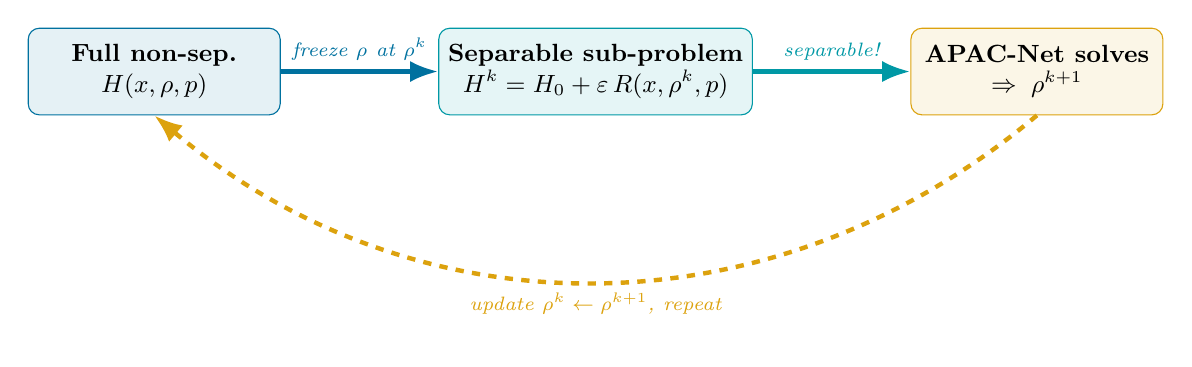
\begin{tikzpicture}[font=\small]
  \node[draw=kaustblue, fill=kaustblue!10, rounded corners, minimum width=3.2cm, minimum height=1.1cm, align=center] (full)
       {\textbf{Full non-sep.}\\$H(x,\rho,p)$};
  \node[right=2cm of full, draw=kaustteal, fill=kaustteal!10, rounded corners,
        minimum width=3.2cm, minimum height=1.1cm, align=center] (sub)
       {\textbf{Separable sub-problem}\\$H^k = H_0 + \eps\,R(x,\rho^k,p)$};
  \node[right=2cm of sub, draw=kaustgold, fill=kaustgold!10, rounded corners,
        minimum width=3.2cm, minimum height=1.1cm, align=center] (out)
       {\textbf{APAC-Net solves}\\$\Rightarrow\;\rho^{k+1}$};
  \draw[-{Latex}, ultra thick, kaustblue]
       (full)--node[above, font=\scriptsize\itshape]{freeze $\rho$ at $\rho^k$}(sub);
  \draw[-{Latex}, ultra thick, kaustteal] (sub)--node[above, font=\scriptsize\itshape]{separable!}(out);
  \draw[-{Latex}, ultra thick, kaustgold, dashed]
       (out.south) to[bend left=40] node[below, font=\scriptsize\itshape]
       {update $\rho^k\leftarrow\rho^{k+1}$, repeat} (full.south);
\end{tikzpicture}
\end{center}

\medskip
This is a \blue{fixed-point} (Picard) iteration on the density.\\
Each inner solve is a separable MFG that a GAN method handles.
\end{frame}

\begin{frame}{Weakly non-separable Hamiltonians}
\textbf{We define the class:}
\[
  H(x,\rho,p) \;=\;
  \underbrace{H_0(x,p)}_{c_0\text{-convex}}
  \;-\; \underbrace{f_0(x,\rho)}_{\lambda\text{-monotone}}
  \;+\; \eps\,\underbrace{R(x,\rho,p)}_{\text{Lipschitz}}
\]

\medskip
\textbf{Special cases:}
\begin{itemize}\setlength\itemsep{1pt}
  \item $\eps = 0$ recovers the classical \emph{separable} MFG.
  \item $R = \rho\cdot p$ recovers the \emph{traffic-flow} MFG-LWR.
  \item $R = R(x,\rho)$ is the \emph{density-only} subcase.
\end{itemize}

\medskip
\begin{resultbox}[title=GAN-tractable regime]
\centering
\[
  \boxed{\;\eps\,L_R \;<\; \lambda\;}
\]
(plus a companion second condition when $R$ depends on $p$)
\end{resultbox}

\medskip
The threshold balances \emph{coupling strength} against
\emph{Lasry--Lions restoring force}.
\end{frame}

\begin{frame}{The Extended-MFGAN algorithm}
\begin{tcolorbox}[colback=kaustblue!5, colframe=kaustblue, arc=3pt]
\textbf{Outer fixed-point iteration.}
\begin{enumerate}\setlength\itemsep{2pt}
  \item Initialise $\rho^0 \leftarrow \rho_0$.
  \item For $k = 0, 1, \ldots, K-1$:
    \begin{enumerate}
      \item Build $H^k(x,p) = H_0(x,p) + \eps\,R(x,\rho^k(x,t),p)$.
      \item Run an inner \alert{GAN solver} (e.g.\ APAC-Net) on the
            separable MFG with $H^k$:
            $(\varphi^{k+1},\rho^{k+1}) \leftarrow \textsc{APAC-Net}(H^k,f_0,g,\rho_0)$.
    \end{enumerate}
  \item Return $(\varphi^K,\rho^K)$.
\end{enumerate}
\end{tcolorbox}

\medskip
\textbf{Sanity check.}  At $\eps=0$, $H^k\equiv H_0$, the outer loop
converges in \emph{one} step, and we recover APAC-Net exactly.

\medskip
\textbf{Cost.}  $K$ APAC-Net runs.  Once we prove the contraction rate
$\kappa$, we have $K = \lceil \log(1/\delta)/\log(1/\kappa)\rceil$ for
target accuracy $\delta$.
\end{frame}

\begin{frame}{Our main theorem: $L^2$ contraction}
\begin{resultbox}[title=Theorem (Wasserstein contraction)]
Under Lasry--Lions monotonicity ($\lambda$), strong convexity of $H_0$
($c_0$), bounded densities, and the GAN-tractable condition,
the outer iteration satisfies
\[
  \|\rho^{k+1}-\rho^*\|_{L^2} \;\leq\; \kappa\;\|\rho^k-\rho^*\|_{L^2},
  \qquad
  \boxed{\;\kappa = \dfrac{\eps L_R}{\lambda}\;}
\]
\textbf{Corollary.}  $\rho^k \to \rho^*$ in $\mathcal{W}_2$ at rate
$\kappa^{k/2}$ (from the $L^2$-to-$\W_2$ inequality).
\end{resultbox}

\medskip
\textbf{This is the first explicit convergence rate for a deep
MFG solver in the non-separable setting.}\\
Proven via the \blue{Lasry--Lions duality identity}.

\medskip
\textbf{Sharpness (additional theorem).}  The rate is \emph{tight}:
on the bilinear traffic-flow family at the uniform equilibrium,
the linearised outer map has operator norm exactly $\eps|1-\eps|/\lambda$.

\medskip
\textbf{Necessity (additional theorem).}  When $\eps L_R \geq \lambda$,
the iteration diverges (explicit linearised counterexample).
\end{frame}

\begin{frame}{Comparison: where we sit}
\begin{center}
\renewcommand{\arraystretch}{1.4}
\begin{tabular}{lcccc}
\toprule
& Non-sep.\ $H$ & $\rho$ rep. & Convergence & Rate \\
\midrule
APAC-Net / MFGAN  & \xmark & \teal{distributional} & $\W_1$ & \xmark \\
MFDGM \scriptsize(\citehl{Assouline--Missaoui 2023})
                  & \cmark & \alert{pointwise NN}  & $L^p,\,p<2$ & \xmark \\
\rowcolor{kaustteal!12}
\textbf{Extended-MFGAN (ours)}
                  & \cmark{\scriptsize\,(weakly)} &
                    \teal{distributional} &
                    $L^2$ and $\W_2$ &
                    \blue{$\kappa^k$} \\
\bottomrule
\end{tabular}
\end{center}

\medskip
\textbf{We close all three gaps within the weakly non-separable regime.}

\medskip
\textbf{Trade-off.}  We are restricted to $\eps L_R<\lambda$.\\
Outside this regime, MFDGM remains preferred.
\end{frame}

\begin{frame}{Summary}
\textbf{The paper of \citehl{Assouline--Missaoui 2023}:}
\begin{itemize}\setlength\itemsep{1pt}
  \item Two networks, PINN-style residual minimisation.
  \item Works for \emph{any} Hamiltonian, including MFG-LWR.
  \item Scales to $d=300$ with a single hidden layer.
  \item Convergence in $L^p$ for $p<2$, no rate.
\end{itemize}

\medskip
\textbf{Our extension:}
\begin{itemize}\setlength\itemsep{1pt}
  \item Define \emph{weakly non-separable} Hamiltonians.
  \item \blue{Freeze $\rho$} to make each subproblem separable
        $\Rightarrow$ inner GAN solver applies.
  \item Prove $L^2$ contraction with explicit rate
        $\kappa = \eps L_R/\lambda$.
  \item Wasserstein-2 convergence at rate $\kappa^{k/2}$.
  \item Sharp threshold $\eps L_R<\lambda$, both necessary and sufficient.
\end{itemize}

\medskip
\teal{Both methods are complementary, not competing.}
\end{frame}

%% =================================================================
%%  THANK YOU
%% =================================================================
{
\setbeamercolor{background canvas}{bg=kaustblue}
\setbeamercolor{normal text}{fg=white}
\begin{frame}[plain]
\usebeamercolor[fg]{normal text}
\centering
\vspace{0.6cm}
{\Huge\textbf{Thank you}}\\[6pt]
{\Large Questions?}

\vspace{0.5cm}
\textcolor{kaustgold}{\rule{0.35\textwidth}{0.6pt}}
\vspace{0.4cm}

{\itshape Deep Learning for Mean Field Games\\
with Non-Separable Hamiltonians}\\[6pt]
\scriptsize\,Assouline \& Missaoui (\emph{Chaos, Solitons \& Fractals}, 2023)\\[16pt]

{\normalsize Today's reader: Hikmatullo Ismatov}\\
{\small\textsl{King Abdullah University of Science and Technology}}\\[10pt]

{\small\ttfamily hikmatullo.ismatov@kaust.edu.sa}
\end{frame}
}

\end{document}
